\documentclass[10pt,letterpaper]{article}
%\usepackage{times}
\usepackage[margin=1in,hmargin=1in]{geometry}
\usepackage{amsmath}
\usepackage{tikz,url}
\usepackage{amssymb}
\usepackage{fancyhdr}
\usetikzlibrary{matrix}
\usepackage{listings}
\usepackage{tabularx}
\usepackage{xcolor}
\usepackage{graphicx}
\usepackage{graphics}
\usepackage{titling}
\pagestyle{fancy}
\usepackage{float}
\usepackage{fancyvrb}
\usepackage{verbatim}
\usepackage{enumitem}
%\usepackage{float}
%\restylefloat{table}

\fancyhead[LO]{STAT W4201 Advanced Data Analysis}
\fancyhead[RO]{HW 4}
\fancyhead[LE]{STAT W4201 Advanced Data Analysis}
\fancyhead[RE]{HW 4}
\title{\textbf {Homework 4}}
\author{{Qianbo Wang}\\{uni: qw2180}}
\date{}
\setlength{\droptitle}{-5em}
\setlength{\parindent}{0pt}

\makeatletter
\newcommand{\rmnum}[1]{\romannumeral #1}
\newcommand{\Rmnum}[1]{\expandafter\@slowromancap\romannumeral #1@}
\makeatother

\lstset{
language=R,
tabsize=4, 
%frame=shadowbox, 
commentstyle=\color{red!50!green!50!blue!50},
%rulesepcolor=\color{red!20!green!20!blue!20},
keywordstyle=\color{blue!90},
showstringspaces=false,
stringstyle=\ttfamily, 
keepspaces=true, 
breakindent=22pt, 
numbers=none,
stepnumber=1,
numberstyle=\tiny, 
numberstyle={\color[RGB]{0,192,192}\tiny} ,
numbersep=5pt,  
basicstyle=\footnotesize, 
showspaces=false, 
flexiblecolumns=true, 
comment=[l]{\#},
texcl=true,
escapeinside={\$$}{\^^M},
breaklines=true, 
breakautoindent=true,
breakindent=4em, 
aboveskip=1em, 
tabsize=2,
showstringspaces=false, 
backgroundcolor=\color[RGB]{244,244,244},   
fontadjust,
captionpos=t,
framextopmargin=2pt,framexbottommargin=2pt,abovecaptionskip=-3pt,belowcaptionskip=3pt,
extendedchars=false,columns=flexible
}

\begin{document}
\maketitle
\thispagestyle{fancy}
\vspace{-2em}
{\large{\textbf{Consider the Boston dataset, in R library MASS, on Housing Values in Suburbs of Boston.}}}
\begin{enumerate}[leftmargin=0cm,itemindent=.5cm,labelwidth=\itemindent,labelsep=0cm,align=left]
\item[(a). ] Fit a multiple linear regression model to predict medv (median value of owner-occupied homes in \$1000s) using the following set of predictors: crim, zn, indus, nox, rm, age, tax.

The linear regression result is as follows:
\begin{center}
Multiple linear regression result 
\verbatiminput{lsresult.txt}
\end{center}

The multiple linear regression is:  \[medv = -19.62 - 0.13crim + 0.02zn - 0.01indus + 0.1nox + 7.61rm - 0.02age - 0.01tax\] 
And the simple t-test results on the parameters are as follows: 
\begin{center}
Test on coefficients result 
\verbatiminput{multilinear.txt}
\end{center}

Since from the result we can find that use t-test on whether the coefficient is 0, there are 4 variables that are not significant under $5\%$ significance level, including zn, indus, nox, and age. The $R^2 = 0.5818$ and the adjusted $R^2 = 0.576$, which is not very good.  
The following is the plot of the residuals and fitted values: \\
\begin{center}
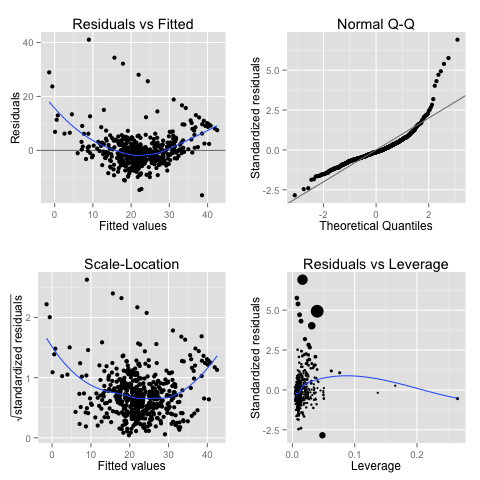
\includegraphics[scale=0.8]{multilinear}
\end{center}

\item[(b). ] State and assess the validity of the underlying assumptions, and suggest remedial measures in case of violations of any of the underlying assumptions.\\
\begin{enumerate}[leftmargin=0cm,itemindent=.5cm,labelwidth=\itemindent,labelsep=0cm,align=left]
\item[\textbullet]Linearity/functional form 
\item[\textbullet]Normality 
\item[\textbullet]Homoscedasticity 
\item[\textbullet]Uncorrelated error
\end{enumerate}

\begin{enumerate}[leftmargin=0cm,itemindent=.5cm,labelwidth=\itemindent,labelsep=0cm,align=left]
\item[1.] Linearity/functional form
\begin{enumerate}[leftmargin=0cm,itemindent=.5cm,labelwidth=\itemindent,labelsep=0cm,align=left]
\item[(1). ] Plot the scatter plot of the response vs. explanatory variables. 

From the scatter plot we can find that for the explanatory variable zn, indus, nox and tax, the scatter plot is a mess. Since the regression is not a straight line and is not monotonic, and the variablity of response is about the same at all values of x,  then we should either try quadratic form or exclude the explanatory variables because the linear form doesn't make sense.\\
\begin{center}
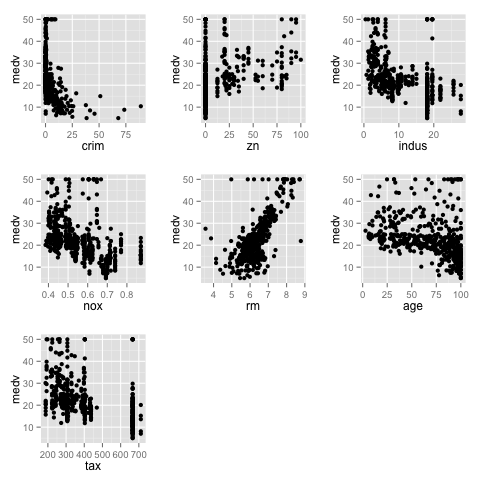
\includegraphics[scale=0.8]{scatter1}
\end{center}
 
\item[(2). ] Compute $R^2$.

Since $R^2=0.5818$, and adjust $R^2 = 0.576$, which is small, then this indicates that the model doesn't fit well on the data, i.e. the response data and explanatory data are not well-fitted linear association. \\

\item[(3). ] Plot the residuals vs. fitted values. 

Since from the plot we can see that most of the residuals are around x-line, except several outliers, and the outliers are extremely large, which affect much on the regression line. And this indicates that the regression line is not strictly a linearity/functional form. And the residuals are horn-shaped, then we should do some transform on y, such as logarithm and take reciprocal. \\

\begin{center}
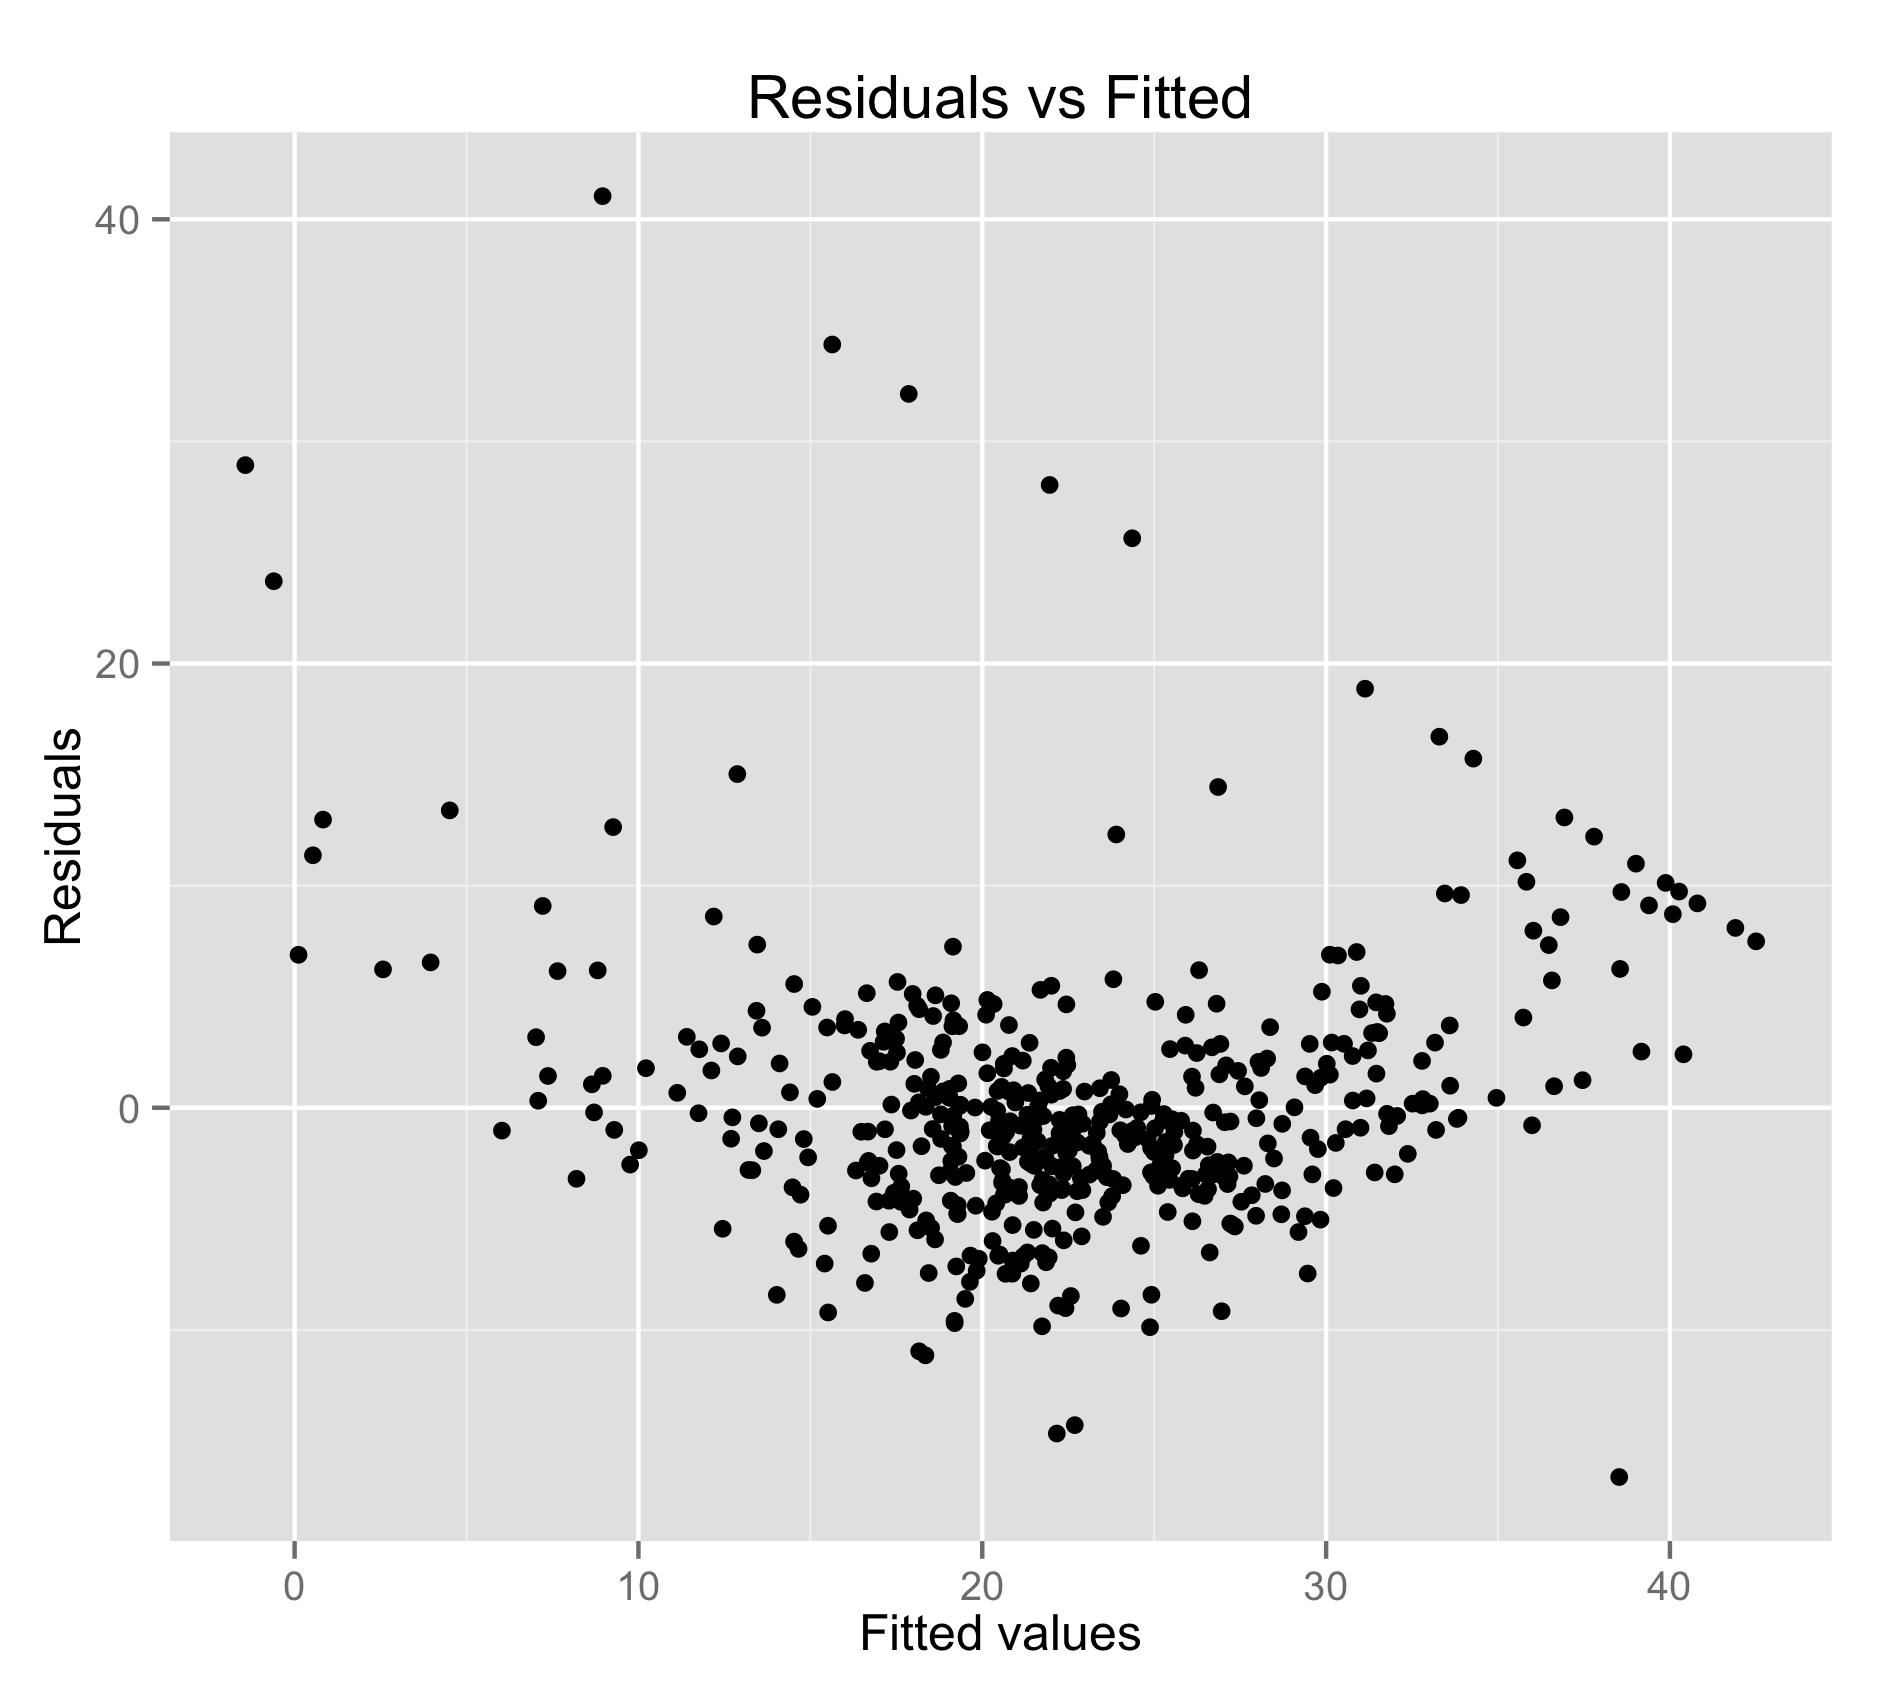
\includegraphics[scale=0.16]{resid}
\end{center}

\item[(4). ] Remedies 

Since the three results conclude that the response and explanatory variables are not linearly form relation. So we should transform the data and exclude some variables, and we can also try some non-linear form on the data or try some new predictors.
\end{enumerate}

\item[2. ] Normality
\begin{enumerate}[leftmargin=0cm,itemindent=.5cm,labelwidth=\itemindent,labelsep=0cm,align=left]
\item[(1). ] Plot the histogram of residuals

Since from the histogram of the residuals we can see that the residuals are skew to the right and there are some outliers in the plot. So these conclude that the residuals are not strictly satisfying normal distribution. 
\begin{center}
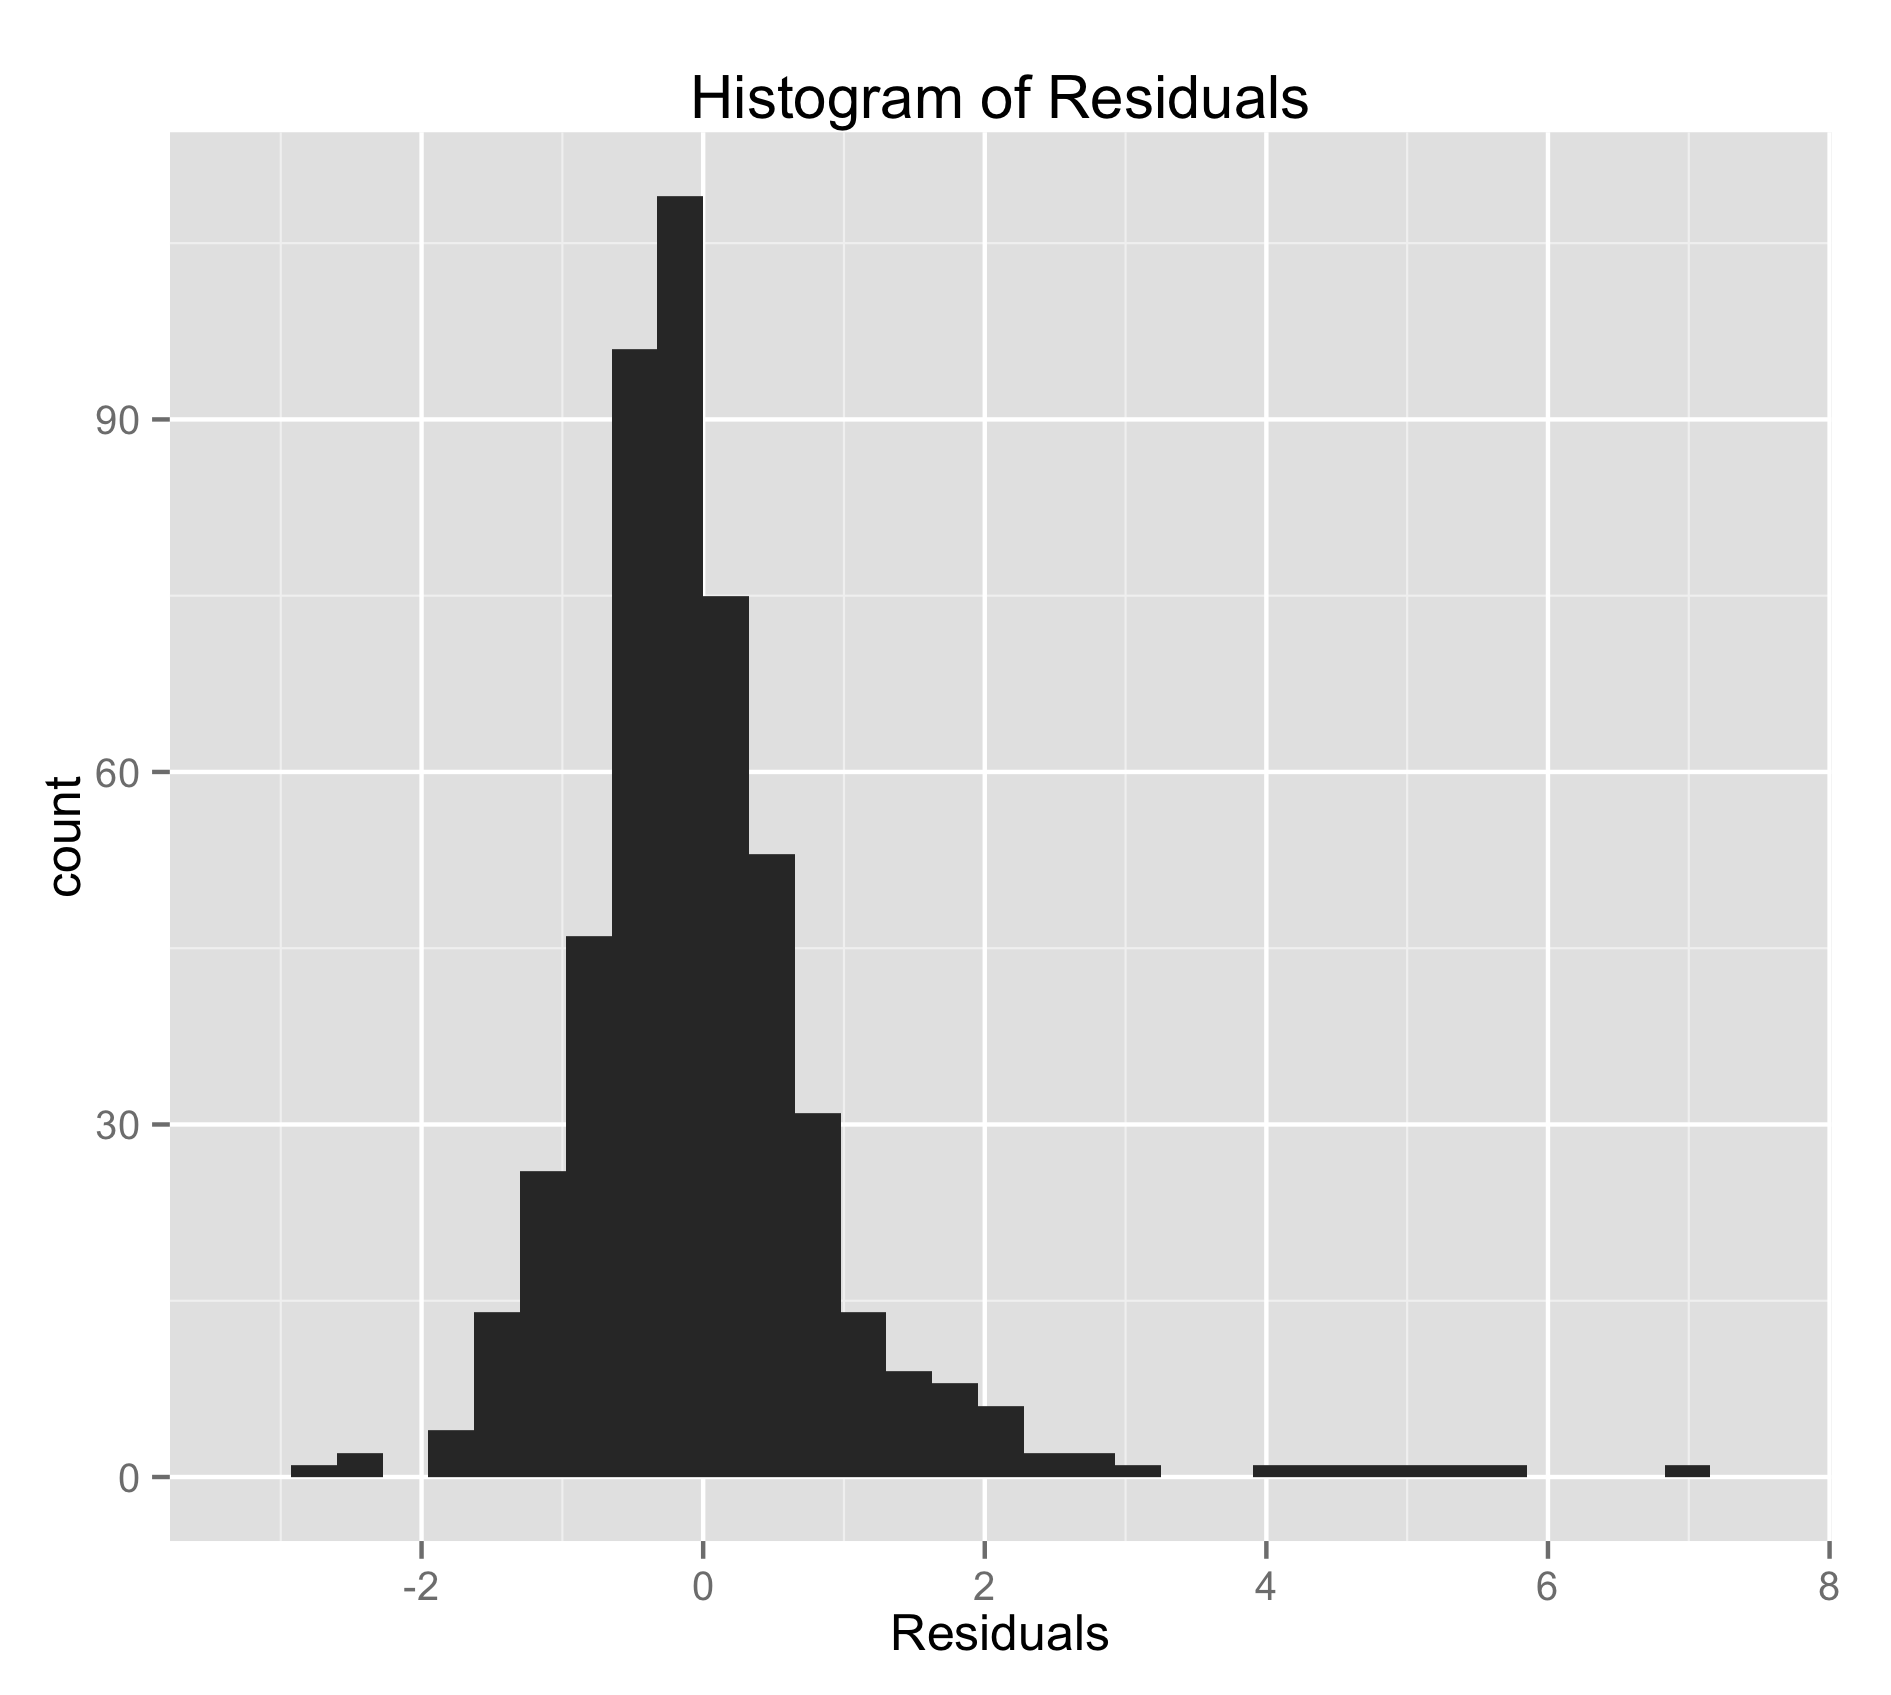
\includegraphics[scale=0.16]{residhist}
\end{center}

\item[(2). ] Plot the Q-Q plot of standardized residuals

From the Q-Q plot of the residuals we can see that the residuals are not located close around the $y=x$ line, in fact, most of the residuals depart far from that line. So we can conclude that the residuals are not normally distributed.
\begin{center}
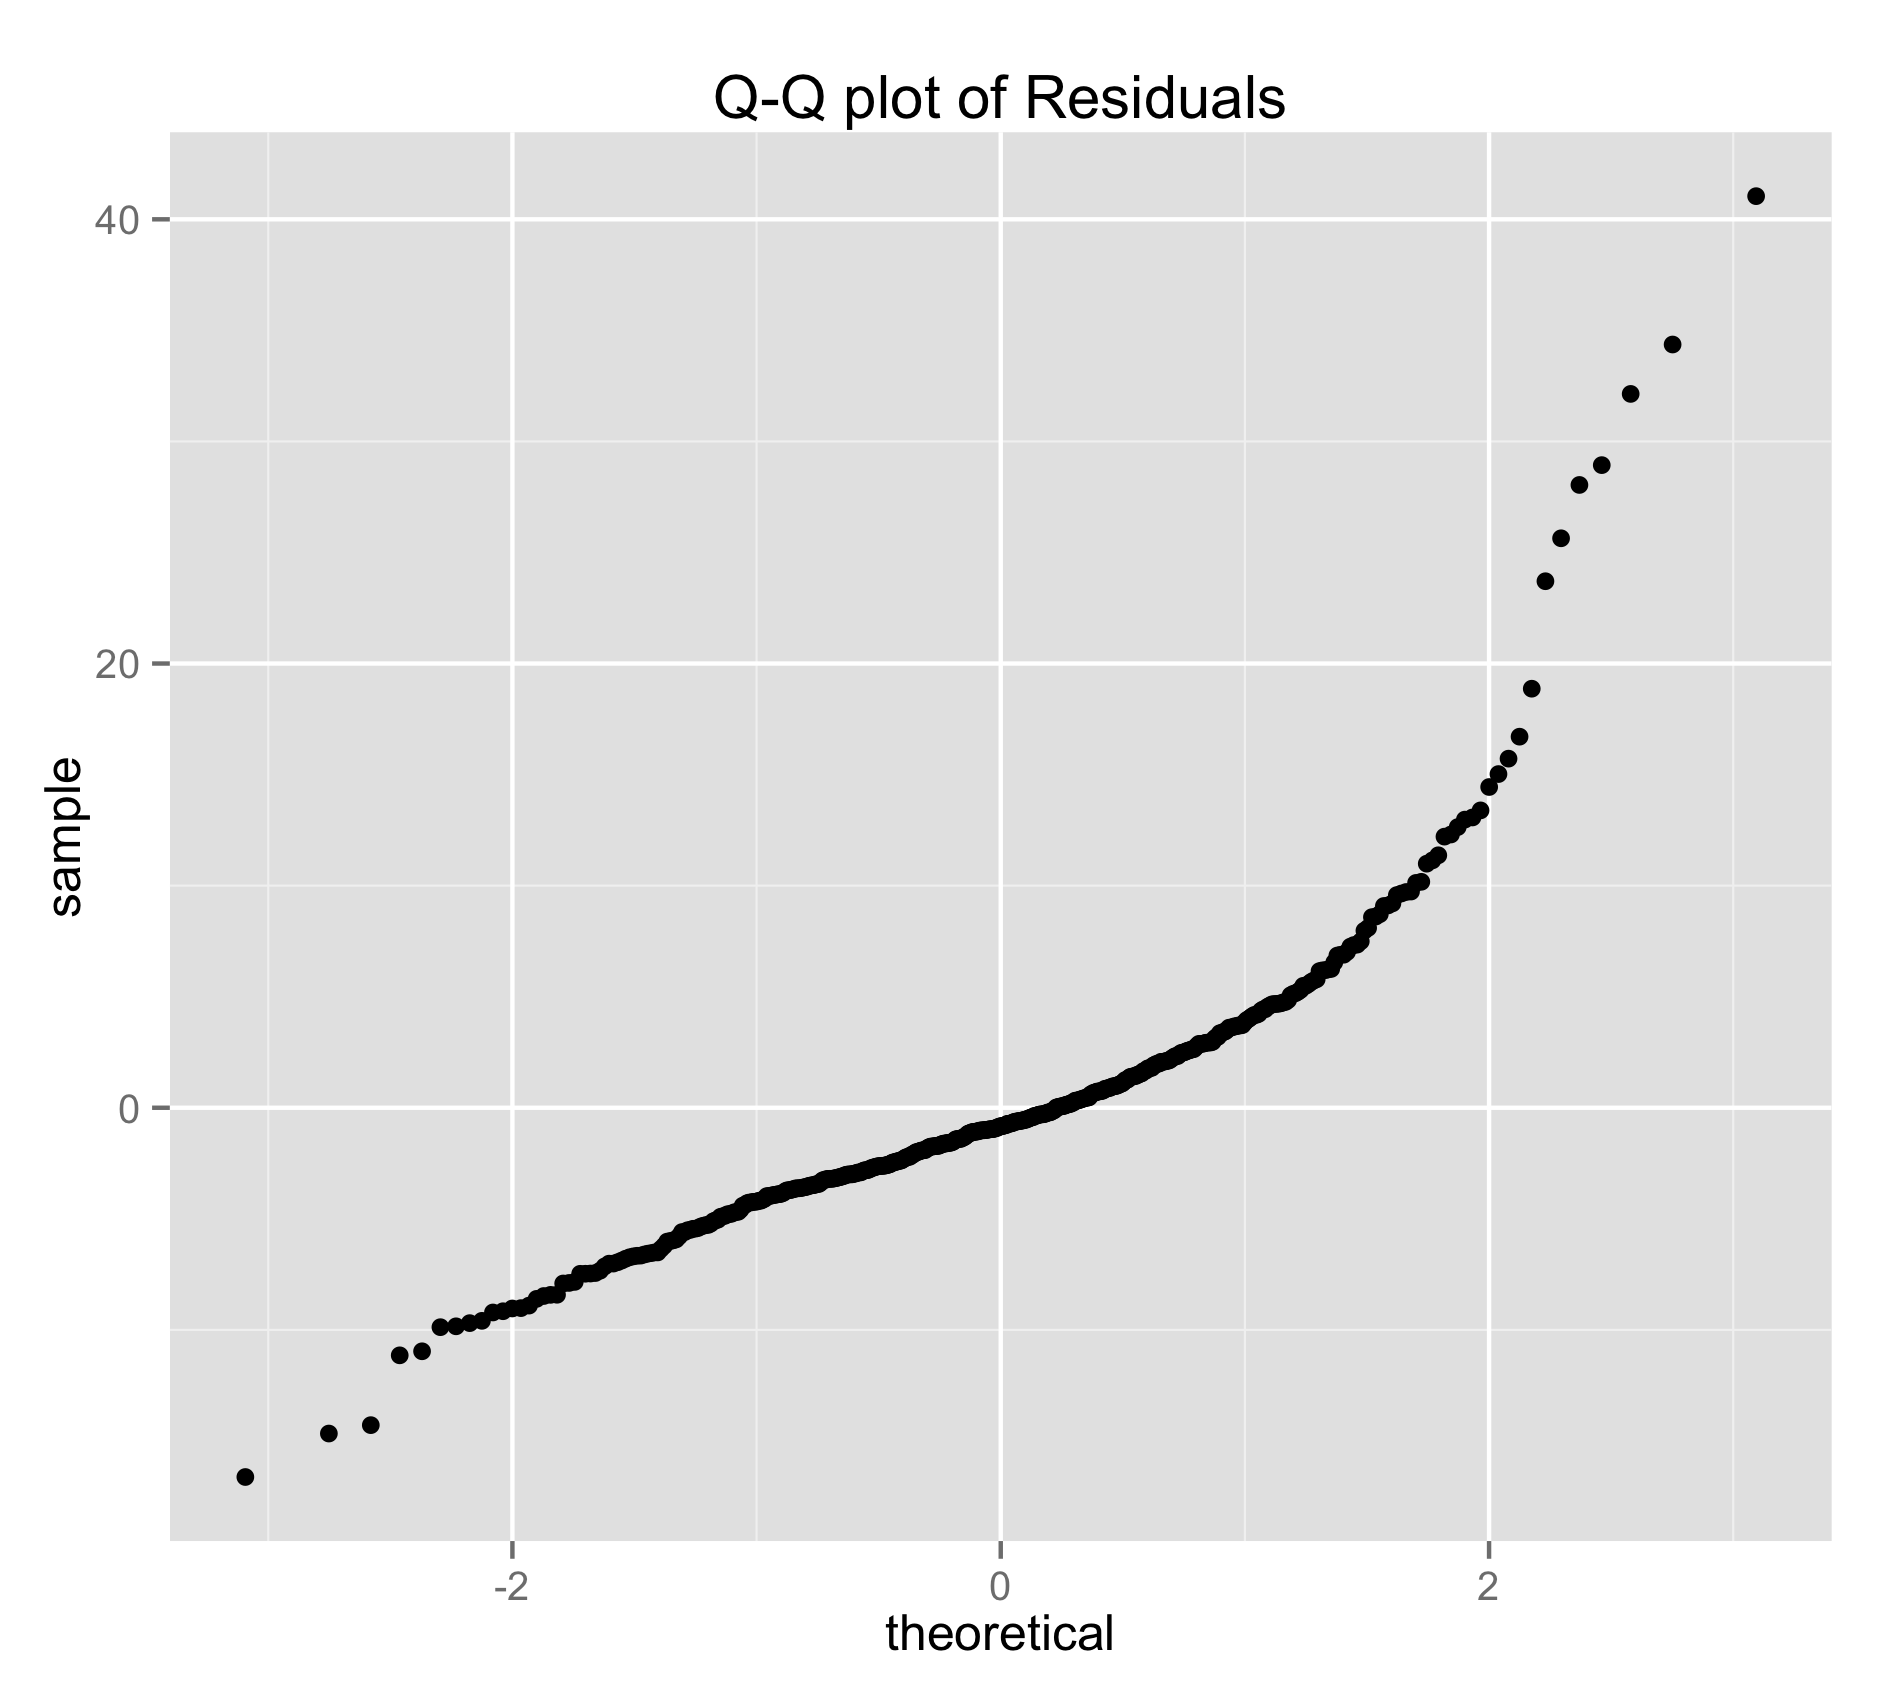
\includegraphics[scale=0.16]{residqq}
\end{center}

\item[(3). ] Shapiro test on residuals 

The hypothesis of shapiro test is : \[H_0: residuals \sim Normal\] 
\[H_1: residuals \ not \ \sim Normal\]
\noindent Since from the result of shapiro test, the $p-value<2.2*10^-16$, then we should reject the null, and conclude that the residuals are not satisfying normal distributions.\\
\begin{center}
Shapiro test on residuals result 
\verbatiminput{shapiro.txt}
\end{center}

\item[(4). ] Remedies 

Since the three results conclude that the data are not satisfying normal distribution. Then we should take transform on data and also try some robust regression method.\\
\end{enumerate}

\item[3. ] Homoscedasticity 

\begin{enumerate}[leftmargin=0cm,itemindent=.5cm,labelwidth=\itemindent,labelsep=0cm,align=left]
\item[(1). ] Plot the scatter plot of residuals vs. explanatory variables. 

From the plot we can see that none of the 7 explanatory variables are satisfying homoscedasticity, all of them are not constant variance around the line.\\

\begin{center}
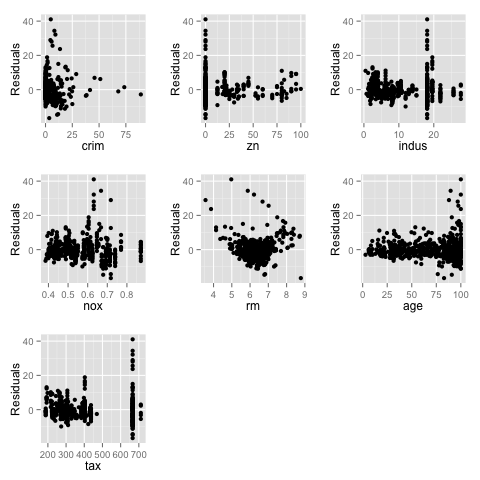
\includegraphics[scale=0.8]{residx}
\end{center}

\item[(2). ] Remedies 

Since the plot result conclude that the data are not satisfying homoscedasticity. So we should transform the data. And also, we can try weighted least sum of squares since the data residuals are non-constancy variance, we can assemble different weight on them and solve the problem.\\
\end{enumerate}

\item[4. ] Uncorrelated error
\begin{enumerate}[leftmargin=0cm,itemindent=.5cm,labelwidth=\itemindent,labelsep=0cm,align=left]
\item[(1). ] Durbin-Watson Test 

The hypothsis of dw test are: \[H_0: \rho = 0\] 
\[H_1: \rho \neq 0\]
From the dw test result, we can see that $p-value = 0$, which indicates that there are  correlated errors in this regression.\\

\begin{center}
Durbin-Watson Test Result
\verbatiminput{dwtest.txt}
\end{center}

\item[(2). ] Remedies 

Since there are correlated errors, we should use Cochrane-Orcutt Procedure to do transform on data, and also use some models that incorporate the correlation structure such as Generalized Estimating Equations, to avoid the correlated errors.
\end{enumerate}

\item[5. ] Remedies to take
\begin{enumerate}[leftmargin=0cm,itemindent=.5cm,labelwidth=\itemindent,labelsep=0cm,align=left]
\item[\textbullet] non-linearility

For response,  a horn-shaped residuals vs fitted plot indicates that we should transform on response, use logarithm. Plot new scatter plots on transformed response and explanatory variables. From the plot we can see some remedies on x. \\
For crim we should try reciprocal of y, because the regression is not a straight line and is monotonic, though some outliers and the variablity of response is decreasing with x increasing, then we don't need transform data\\
For zn, since there is no need to transform the data, because the regression is not a straight line and is not monotonic, and the variablity of response is not monotic with x increasing. Then we can try some quadratic form on zn.\\
For indus, since the regression is not a straight line and is monotonic decreasing, though some outliers and the variablity of response is not monotonic with x increasing, then we don't need transform data.\\
For nox, since the regression is not a straight line and is monotonic, though some outliers and the variablity of response is increasing with x increasing, then we can take the logarithm on x\\
For age, since the regression is not a straight line and is not monotonic, and the variablity of response is increasing with x increasing, then we can take some transform on x, take the reciprocal.\\
For tax, since the regression is not a straight line and is not monotonic, it is a mess and the variablity of response is about the same with x increasing, then we don't need transform on tax, i.e. exclude it from the model.\\
\begin{center}
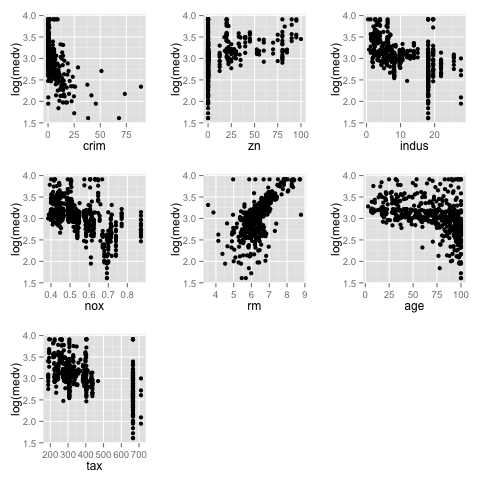
\includegraphics[scale=0.8]{transform}
\end{center}

\item[\textbullet] non-normality

Since from the first part, we have took logrithm on the data, and this time we should try some robust regression method, such as least median of squares, not the ordinary least of sum of squares method.\\

\item[\textbullet] non-homoscedasticity

Since from the first part, we have took logrithm on the data, and the result is still not good.Then we should try weighted method on the data, since non-constancy-variance, then we just assign weights to make sure the weighted variance equal.

\item[\textbullet] correlated-errors

Use models that incorporate the correlation structure such as Generalized Estimating Equations.
\end{enumerate}
\end{enumerate}

\item[(c). ] Repeat (a) using Least Median of Squares Regression and compare the results with those obtained in (a).

The Least Median of Squares regression result is as follows:
\begin{center}
Multiple linear regression result 
\verbatiminput{lmsresult.txt}
\end{center}

The least median of squares regression is:  \[medv = -27.99 - 0.71crim + 0.03zn + 0.02indus + 3.70nox + 8.02rm - 0.04age - 0.001tax\] 
Compare the two results from (a) and (c). 

\begin{table}[h]
\caption{The coefficients of least sum of square and least median of square}
\centering
\begin{tabular*}{0.9\linewidth}{@{\extracolsep{\fill}}ccccccccc}
\hline 
 & intercept & crim & zn & indus & nox & rm & age & tax \\
\hline
sum of square & -19.62 & -0.13 & 0.02 & -0.01 & 0.1 & 7.61 & -0.02 & -0.01\\
\hline
median of square & -27.99 & -0.71 & 0.03 & 0.02 & 3.70 & 8.02 & -0.04 & -0.001\\
\end{tabular*}
\end{table}

From the table we can see that the coefficients are approximately close, but on intercept, crim, indus and tax, there are significantly differences between the two models.
\end{enumerate}

\newpage
\textbf{R Code: }
\begin{lstlisting}
rm(list=ls())
library(MASS)
library(ggplot2)
#delete containing na value rows
Boston <- na.omit(Boston)

multilinear <- lm(medv ~ crim+zn+indus+nox+rm+age+tax, data=Boston)
sink("/Users/Qianbo/Downloads/HW4/lsresult.txt")
multilinear
sink()
sink("/Users/Qianbo/Downloads/HW4/multilinear.txt")
summary(multilinear)
sink()

#plot the mulilinear regression 
plot1<-ggplot(multilinear,aes(.fitted,.resid))+
  geom_hline(yintercept=0,color="grey50",size=0.5)+
  geom_point()+geom_smooth(size=0.5,se=FALSE)+
  ggtitle("Residuals vs Fitted")+xlab("Fitted values")+ylab("Residuals")

plot2<-ggplot(multilinear,aes(sample=.stdresid))+
  stat_qq()+geom_abline(color="grey50")+
  ggtitle("Normal Q-Q")+
  ylab("Standardized residuals")+xlab("Theoretical Quantiles")

plot3<-ggplot(multilinear,aes(.fitted,sqrt(abs(.stdresid))))+
  geom_point()+geom_smooth(se=FALSE)+
  ggtitle("Scale-Location")+
  xlab("Fitted values")+ylab(expression(sqrt("standardized residuals")))

plot4<-ggplot(multilinear,aes(.hat,.stdresid,size=.cooksd))+
  geom_point()+geom_smooth(se=FALSE,size=0.5)+
  ggtitle("Residuals vs Leverage")+scale_size_continuous(guide=FALSE)+
  xlab("Leverage")+ylab("Standardized residuals")

library(grid)
library(gridExtra)

grid.arrange(plot1,plot2,plot3,plot4,ncol=2)
png("/Users/Qianbo/Downloads/HW4/multilinear.png")
grid.arrange(plot1,plot2,plot3,plot4,ncol=2)
dev.off()

#check assumptions
#check Linear/functional form
#scatter plot of y vs x
s1<-ggplot(Boston,aes(crim,medv))+geom_point()
s2<-ggplot(Boston,aes(zn,medv))+geom_point()
s3<-ggplot(Boston,aes(indus,medv))+geom_point()
s4<-ggplot(Boston,aes(nox,medv))+geom_point()
s5<-ggplot(Boston,aes(rm,medv))+geom_point()
s6<-ggplot(Boston,aes(age,medv))+geom_point()
s7<-ggplot(Boston,aes(tax,medv))+geom_point()

png("/Users/Qianbo/Downloads/HW4/scatter1.png")
grid.arrange(s1,s2,s3,s4,s5,s6,s7,ncol=3)
dev.off()

#scatter plot of residuals vs fitted 
residplot<-ggplot(multilinear,aes(.fitted,.resid))+
  geom_point()+ggtitle("Residuals vs Fitted")+
  xlab("Fitted values")+ylab("Residuals")
ggsave('/Users/Qianbo/Downloads/HW4/resid.png')

#check Normality
#histogram of residuals
hist<-ggplot(multilinear,aes(.stdresid))+
  geom_histogram()+ggtitle("Histogram of Residuals")+xlab("Residuals")
hist
ggsave(file="/Users/Qianbo/Downloads/HW4/residhist.png")

#qq plot of standardized residuals
qqresid<-ggplot(multilinear,aes(sample=.stdresid))+
  stat_qq()+geom_abline(aes(intercept=0,scope=1),color="grey50",size=0.5)+
  ggtitle("Q-Q plot of std Residuals")
qqresid
ggsave(file="/Users/Qianbo/Downloads/HW4/residqq.png")

#shapiro test on residuals
residuals = resid(multilinear)
shapiro.test(residuals)
sink("/Users/Qianbo/Downloads/HW4/shapiro.txt")
shapiro.test(residuals)
sink()

#check Homoscedasticity
#scatter plot of residuals vs x
r1<-ggplot(multilinear,aes(crim,.resid))+geom_point()+ylab("Residuals")
r2<-ggplot(multilinear,aes(zn,.resid))+geom_point()+ylab("Residuals")
r3<-ggplot(multilinear,aes(indus,.resid))+geom_point()+ylab("Residuals")
r4<-ggplot(multilinear,aes(nox,.resid))+geom_point()+ylab("Residuals")
r5<-ggplot(multilinear,aes(rm,.resid))+geom_point()+ylab("Residuals")
r6<-ggplot(multilinear,aes(age,.resid))+geom_point()+ylab("Residuals")
r7<-ggplot(multilinear,aes(tax,.resid))+geom_point()+ylab("Residuals")

grid.arrange(r1,r2,r3,r4,r5,r6,r7,ncol=3)
png("/Users/Qianbo/Downloads/HW4/residx.png")
grid.arrange(r1,r2,r3,r4,r5,r6,r7,ncol=3)
dev.off()

#check Corrected errors
#dw test
library(car)
durbinWatsonTest(multilinear)
sink("/Users/Qianbo/Downloads/HW4/dwtest.txt")
durbinWatsonTest(multilinear)
sink()
#remedies 
#transform on data 
n1<-ggplot(Boston,aes(crim,log(medv)))+geom_point()
n2<-ggplot(Boston,aes(zn,log(medv)))+geom_point()
n3<-ggplot(Boston,aes(indus,log(medv)))+geom_point()
n4<-ggplot(Boston,aes(nox,log(medv)))+geom_point()
n5<-ggplot(Boston,aes(rm,log(medv)))+geom_point()
n6<-ggplot(Boston,aes(age,log(medv)))+geom_point()
n7<-ggplot(Boston,aes(tax,log(medv)))+geom_point()

png("/Users/Qianbo/Downloads/HW4/transform.png")
grid.arrange(n1,n2,n3,n4,n5,n6,n7,ncol=3)
dev.off()

# use least median square method do linear regression

lmslinear<-lmsreg(medv ~ crim+zn+indus+nox+rm+age+tax, data=Boston)
sink("/Users/Qianbo/Downloads/HW4/lmsresult.txt")
lmslinear
sink()


\end{lstlisting}

\end{document}